\chapter{Computation Time Study and Bottlenecks}\label{ch:performance}

The approach moves the cost of the microscale from the macroscopic solve into an
offline phase. Its efficiency is therefore decided by a chain of four costs:
(i)~the direct RVE solves that generate the training data, (ii)~the constitutive
evaluation per macroscopic Newton iteration, (iii)~the number of Newton iterations
the macroscopic problem needs, and (iv)~the resulting overall budget compared with
a concurrent FE$^2$ computation. This chapter quantifies each link and identifies
the bottleneck at each stage (\cref{fig:bottlenecks}). Memory is not a limiting
factor at the problem sizes considered: the largest macroscopic model has
83\,628 quadrature points and the RVE systems have at most 7518 unknowns.

All timings are measured by the program itself: by stage
timers built into the bridge (\code{TIMINGS} in \code{src\slash{}ngsolve\_umat.py}),
by the timing benchmark \code{benchmarks\slash{}rve\_surrogate\_rve\_benchmark.py}, and by
the dataset generator. Newton iteration counts are taken from the stored run
reports. No timing was taken by hand.

\begin{figure}[htbp]
\centering
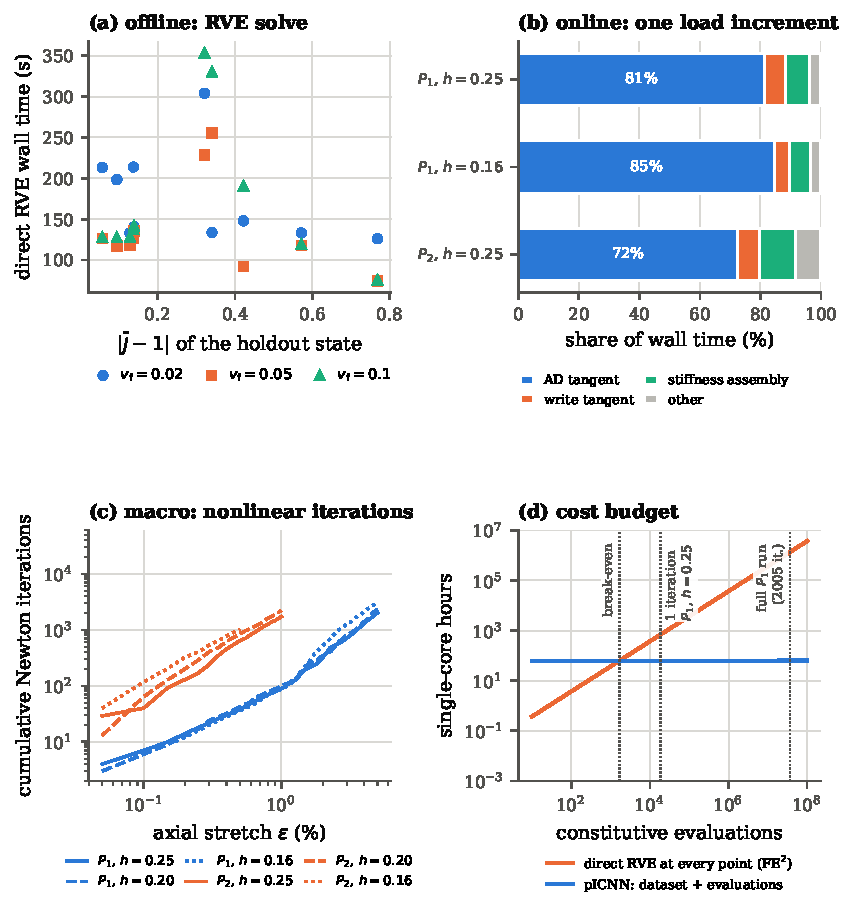
\includegraphics[width=\textwidth]{fig_bottlenecks.pdf}
\caption[Bottlenecks of the approach]{Bottlenecks of the approach. (a) Offline: wall time of one direct RVE
evaluation for the 30 benchmark cases versus the distance $|\overline J-1|$ of the state from
the reference configuration; the spread is not explained by $|\overline J-1|$ (Spearman
$\rho=-0.15$). (b) Online: stage shares of the bridge for the first load increment
(\cref{tab:profile}). (c) Macroscopic solve: cumulative Newton iterations along the
load path of the stored runs ($P_2$, $h=0.16$: run to $0.5\,\%$). (d) Overall budget:
single-core hours for $N$ constitutive evaluations, direct RVE at every evaluation
($134\,$s each, without tangent) versus the surrogate (1671 dataset solves plus
$36\,\mu$s per evaluation including the tangent).}
\label{fig:bottlenecks}
\end{figure}

\section{Offline cost: direct RVE versus surrogate}

The paired benchmark on 30 fresh-holdout cases (one thread, cluster node, two
repeats per direct RVE, fifteen per surrogate) gives the timings in
\cref{tab:timing} and \cref{fig:timing}. One direct RVE evaluation requires the
free-rotation equilibrium plus energy and stress recovery. It takes a median of
$134\,$s, ranging from $75\,$s to $353\,$s depending on the load path and the
continuation steps needed. Mesh generation is negligible ($0.08$--$0.10\,$s per
volume fraction). The surrogate evaluates energy and stress in $2.3\,$ms. The
median paired speed-up is $5.78\times10^4$ (10th--90th percentile
$5.0\times10^4$--$1.1\times10^5$). If the one-off reference-state evaluation of the
network is amortized over the 30 cases, it is $2.7\times10^3$. Generating the
1671-record dataset therefore costs of the order of $1671\times134\,\mathrm{s}\approx62$
single-core hours, before tangents.

\begin{table}[htbp]
\centering\small
\caption{Measured cost of one constitutive evaluation (energy + first Piola stress).}
\label{tab:timing}
\begin{tabular}{@{}lrr@{}}
\toprule
Quantity & Median & Range / note\\
\midrule
direct RVE, $\vfrac=0.02$ & $144\,$s & $126$--$304\,$s\\
direct RVE, $\vfrac=0.05$ & $122\,$s & $75$--$255\,$s\\
direct RVE, $\vfrac=0.10$ & $133\,$s & $76$--$353\,$s\\
pICNN, energy + stress & $2.3\,$ms & per case, 1 thread\\
paired speed-up (solver work) & $5.78\times10^4$ & P10--P90: $5.0\times10^4$--$1.1\times10^5$\\
paired speed-up (incl.\ reference setup) & $2.73\times10^3$ & conservative\\
12-state generation benchmark, 1 vs.\ 12 workers & $1710\,$s / $513\,$s & speed-up $3.3$, efficiency $28\,\%$\\
\bottomrule
\end{tabular}
\end{table}

\begin{figure}[htbp]
\centering
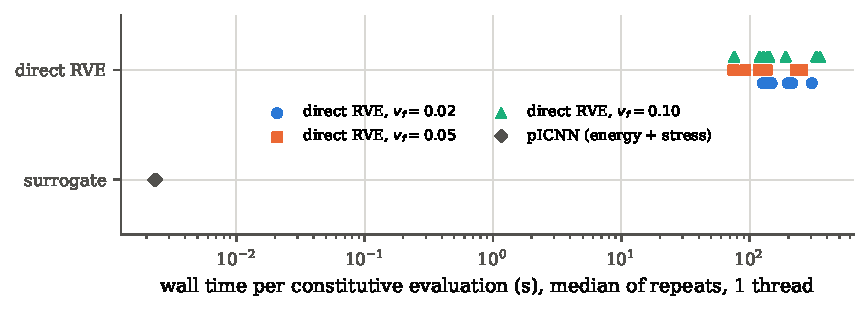
\includegraphics[width=\textwidth]{fig_timing.pdf}
\caption[Wall time per constitutive evaluation, 30 benchmark cases]{Wall time per constitutive evaluation for the 30 benchmark cases: direct
RVE (by volume fraction) versus pICNN. Note the logarithmic axis: the two groups
are separated by almost five decades.}
\label{fig:timing}
\end{figure}

\paragraph{Offline bottleneck.} Dataset generation is the dominant cost of the
whole approach, and its parallel efficiency is low (28\,\% on 12 workers). The
solve times spread by a factor of 4.7 (75--353\,s), and the slowest case takes
2.6 times the median. A few continuation-heavy states therefore dominate the
makespan of a statically partitioned job. \Cref{fig:bottlenecks}(a) shows that
this difficulty cannot be predicted from the size of the deformation: the solve
time is uncorrelated with $|\overline J-1|$. The cost is set instead by the number of
load-continuation steps and rotation updates a state needs, which is known only
after the solve. Sorting the states before distribution would therefore not help.
Dynamic scheduling (a shared work queue with one state per task) is the effective
remedy. The recorded run metadata do not allow start-up and file-system
contributions to be separated from this effect.

\paragraph{Inference.} The surrogate is faster than the direct RVE by a factor of about $2.7\times10^3$ (conservative,
including reference setup) to $5.8\times10^4$ for the constitutive evaluation. This holds for the
tested cases and computing setup only; the saving is real only if many evaluations are needed, because
the data generation is paid once and dominates the total cost.

\section{Online cost: profile of the macroscopic bridge}

\Cref{tab:profile} lists the stage timings for the first load increment of the
macroscopic problem, run with one thread in the local environment
(\code{python -m benchmarks.profile\_bridge}).
This is a separate profiling run; its Newton-iteration counts are those of that run and are not the cluster-run iteration counts of \cref{sec:macro}.

\begin{table}[htbp]
\centering\small
\caption[Built-in stage timings of the bridge, first load increment]{Built-in stage timings of the bridge, first load increment, frozen pICNN, one thread. Shares refer to the total wall time.}
\label{tab:profile}
\begin{tabular}{@{}lrrr@{}}
\toprule
& $P_1$, $h=0.25$ & $P_1$, $h=0.16$ & $P_2$, $h=0.25$\\
\midrule
quadrature points / Newton iterations & 18\,354 / 3 & 83\,628 / 3 & 18\,354 / 25\\
\midrule
1 interpolate and gather $\F$ & $0.6\,\%$ & $0.6\,\%$ & $1.1\,\%$\\
2 pICNN energy, stress, tangent (AD) & $\mathbf{81.4\,\%}$ & $\mathbf{84.7\,\%}$ & $\mathbf{72.4\,\%}$\\
3 write tangent to quadrature points & $6.9\,\%$ & $5.1\,\%$ & $7.3\,\%$\\
4 residual assembly & $0.2\,\%$ & $0.2\,\%$ & $0.3\,\%$\\
5 stiffness assembly & $8.0\,\%$ & $6.8\,\%$ & $11.9\,\%$\\
6 sparse direct solve (UMFPACK) & $0.1\,\%$ & $0.1\,\%$ & $0.8\,\%$\\
other (Python control, line search) & $2.8\,\%$ & $2.6\,\%$ & $6.2\,\%$\\
\midrule
total wall time & $5.7\,$s & $29.7\,$s & $70.4\,$s\\
AD cost per quadrature point & $36\,\mu$s & $43\,\mu$s & $28\,\mu$s\\
\bottomrule
\end{tabular}
\end{table}

\paragraph{Bottleneck.} Between 72 and 85\,\% of the time is spent in the
constitutive evaluation, and almost all of that in the tangent. The nine
reverse-mode passes through a graph with \code{create\_graph=True} cost about
$30$--$40\,\mu$s per quadrature point. Data transfer and assembly together take
about 15\,\%. The sparse solve is negligible at these problem sizes. The cost
scales linearly with the number of quadrature points: $4.6\times$ the points give
$5.5\times$ the AD time. The $P_2$ increment is expensive only because of its 25
Newton iterations (\cref{sec:macro}); per assembly it is as cheap as $P_1$.

\section{Macroscopic solve: number of Newton iterations}

Per iteration, the online cost is small. The total online cost, however, is the
product of this cost and the number of Newton iterations, and the latter is the
bottleneck of the macroscopic stage (\cref{fig:bottlenecks}(c)). The first
increment of the $P_1$ model converges in three iterations, but the iteration count
per step grows along the load path: reaching $5\,\%$ stretch in 100 increments
took 2005, 2318 and 3084 iterations for $h=0.25$, $0.20$ and $0.16$, with up to
47--70 iterations in a single increment. The $P_2$ models need 620--1013
iterations for the first $0.5\,\%$ and 1716--2472 iterations to reach about
$1\,\%$, with up to 194 iterations per increment. The $P_2$ run on the finest mesh
stopped at $0.70\,\%$ when it reached its 24-hour wall-time limit. With the measured
cost of about $1.9\,$s per Newton iteration (seven residual-and-tangent evaluations
in three iterations, \cref{tab:profile}), the $P_1$, $h=0.25$ run corresponds to
roughly one hour of single-core time. The iteration count is driven by
the stiffness ratio $\kappa/\mu\approx10^4$ of the surrogate and by the
conditioning it causes (\cref{sec:macro}), not by the cost of the network. A
faster tangent alone therefore cannot make the $P_2$ runs feasible. The mixed
macroscopic formulation of \cref{sec:proposed} addresses the iteration count
directly.

\paragraph{Inference.} The constitutive evaluation is not the limiting cost of a macroscopic run; the number
of Newton iterations is. An even faster network would therefore change the total cost little, while a
better-conditioned macroscopic formulation would.

\section{Overall cost budget}

\Cref{fig:bottlenecks}(d) combines the offline and online costs. The 1671 dataset
solves cost the same as 1671 direct evaluations, so the surrogate breaks even
after 1671 constitutive evaluations. This is less than one tenth of a single
Newton iteration of the coarsest macroscopic model (18\,354 quadrature points).
The complete $P_1$, $h=0.25$ run evaluated the material law about
$3.7\times10^7$ times. Concurrent FE$^2$ would have needed about $1.4\times10^6$
single-core hours for these evaluations, without the RVE tangents. The surrogate
needed about 63 single-core hours: 62 for generating the data and about one for
the macroscopic run itself.
The training time is not included because it was not recorded consistently;
it does not change the order of magnitude.

\paragraph{Perspective.} One residual-and-tangent evaluation of the $P_1$, $h=0.25$
model costs $\approx0.8\,$s. The corresponding concurrent FE$^2$ iteration on the same mesh would require
18\,354 RVE solves of $\approx134\,$s each, roughly $2.5\times10^6\,$s or about
28~days on one core, still without the RVE tangents. Even with perfect
parallelization on 1000 cores, this would be about 40~minutes per evaluation. The
offline surrogate turns an intractable computation into a seconds-long one. This
is the central benefit of the approach, independent of the accuracy issue of
\cref{sec:diagnosis}.

\paragraph{Summary of the bottlenecks.} Offline, the cost is set by the number
and difficulty of the direct RVE solves, and its parallel execution by load
imbalance. Online, the cost per iteration is set by the AD tangent, and the total
cost by the Newton iteration count of the stiff macroscopic problem. Optimizing
the tangent shortens each iteration by at most a factor of four to seven (the
reciprocal of the non-AD share in \cref{tab:profile}); reducing the
iteration count with a mixed formulation, and the data cost with dynamic
scheduling and active sampling, have the larger potential.

\paragraph{Possible optimizations.} (i) Compute the tangent with a vectorized
Hessian (\code{vmap} over \code{hessian} from \code{torch.func}), or analytically through the
invariants,
\[\Aten=\sum_{a,b}\Psi_{,ab}\,\partial_{\F}y_a\otimes\partial_{\F}y_b
+\sum_a\Psi_{,a}\,\partial^2_{\F}y_a .\]
Only the $4\times4$ Hessian in feature space
then has to come from AD, which should remove most of stage~2. (ii) Write $\Aten$
with a single bulk copy instead of 81 component loops (stage~3). (iii) Reuse the
symbolic structure of the bilinear form across iterations (stage~5).
